\documentclass[../main.tex]{subfiles}

\graphicspath{{\subfix{../images/}}}

\begin{document}

\section{Part 2 - Measurements}

The measured waveforms are shown in Figure \ref{fig:meas-waveforms}, and the critical crosstalk levels are summarized in Tables \ref{tab:meas-side-by-side-microstrip}, \ref{tab:meas-side-by-side-stripline}, and \ref{tab:meas-broadside-stripline}.

\begin{figure}[h]
    \centering
    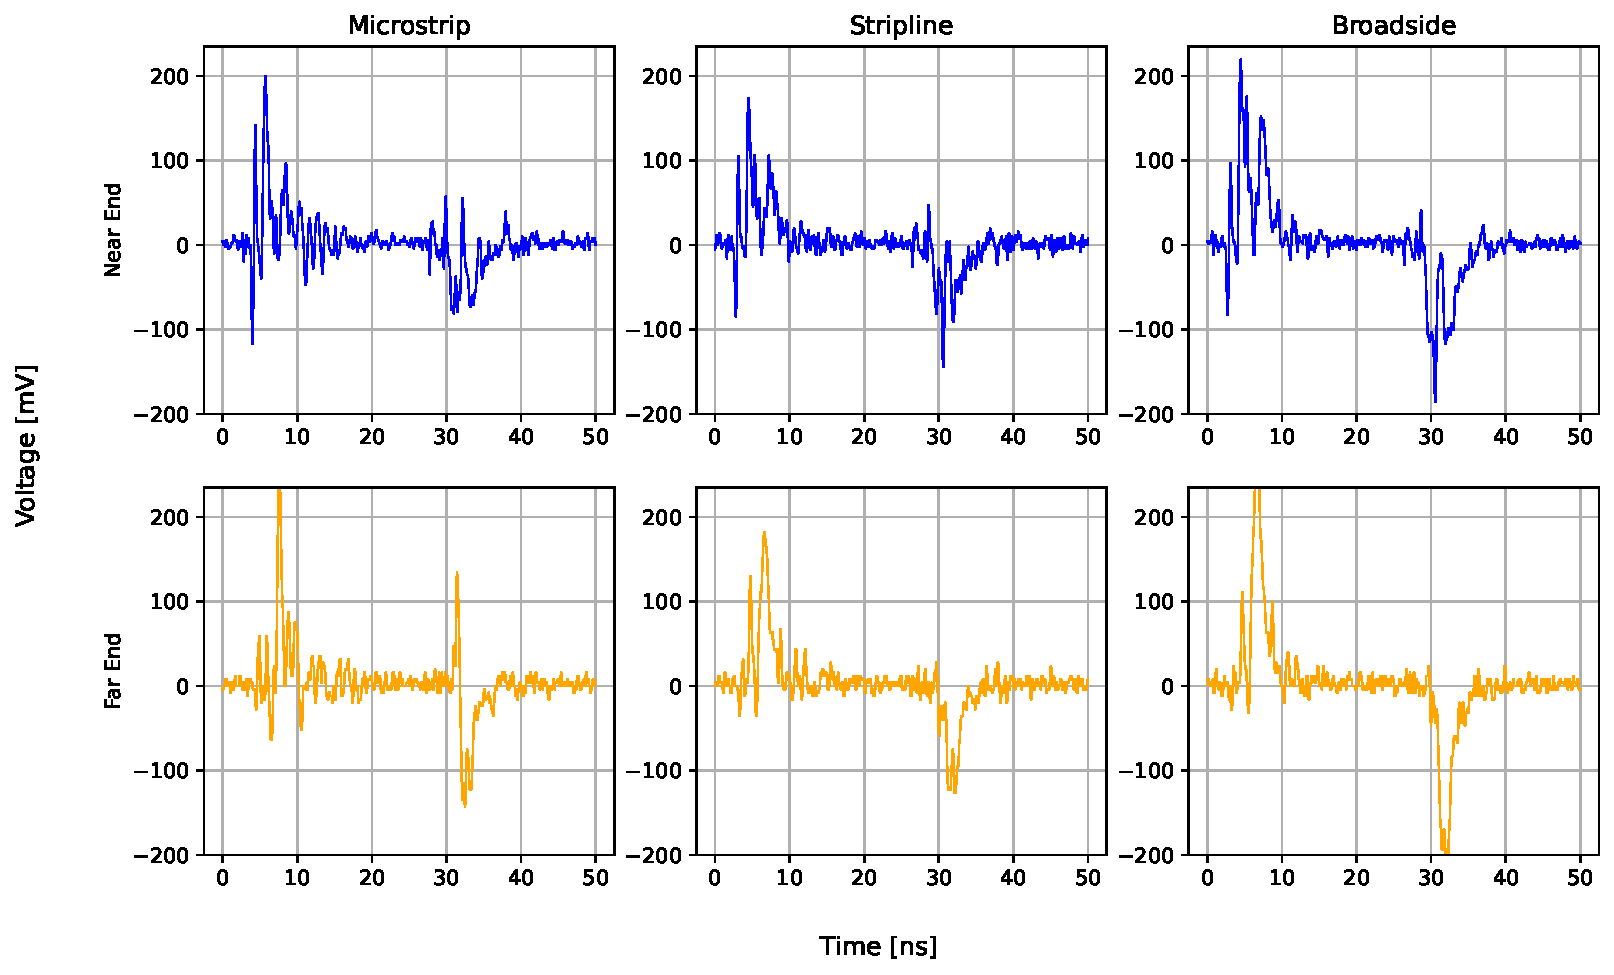
\includegraphics[width=1.0\textwidth]{measured.pdf}
    \caption{Measured waveforms for the three transmission line configurations.}
    \label{fig:meas-waveforms}
\end{figure}

\subsection{Task 2.1 - Crosstalk side-by-side microstrip}

\begin{table}[h]
    \centering
    \begin{tabular}{l l|r r}
        \toprule[1pt]
        \textbf{NEXT} & State & Steady State Level [mV] & Critical Level [mV] \\
        \midrule
        & Low State & 3.51 & 199 \\
        & High State & 3.33 & 3.18 \\
        \midrule[1pt]
        \textbf{FEXT} & State & Steady State Level [mV] & Critical Level [mV] \\
        \midrule
        & Low State & 4.12 & 269 \\
        & High State & 3.32 & 3.16 \\
        \bottomrule[1pt]
    \end{tabular}
    \caption{Crosstalk measurements for side-by-side microstrip.}
    \label{tab:meas-side-by-side-microstrip}
\end{table}

\subsection{Task 2.2 - Crosstalk side-by-side stripline}

\begin{table}[h]
    \centering
    \begin{tabular}{l l|r r}
        \toprule[1pt]
        \textbf{NEXT} & State & Steady State Level [mV] & Critical Level [mV] \\
        \midrule
        & Low State & 2.58 & 174 \\
        & High State & 3.32 & 3.16 \\
        \midrule[1pt]
        \textbf{FEXT} & State & Steady State Level [mV] & Critical Level [mV] \\
        \midrule
        & Low State & 3.62 & 182 \\
        & High State & 3.33 & 3.174 \\
        \bottomrule[1pt]
    \end{tabular}
    \caption{Crosstalk measurements for side-by-side stripline.}
    \label{tab:meas-side-by-side-stripline}
\end{table}

\newpage

\subsection{Task 2.3 - Crosstalk broadside stripline}

\begin{table}[h]
    \centering
    \begin{tabular}{l l|r r}
        \toprule[1pt]
        \textbf{NEXT} & State & Steady State Level [mV] & Critical Level [mV] \\
        \midrule
        & Low State & 3.37 & 219 \\
        & High State & 3.32 & 3.11 \\
        \midrule[1pt]
        \textbf{FEXT} & State & Steady State Level [mV] & Critical Level [mV] \\
        \midrule
        & Low State & 3.59 & 277 \\
        & High State & 3.32 & 3.08 \\
        \bottomrule[1pt]
    \end{tabular}
    \caption{Crosstalk measurements for broadside stripline.}
    \label{tab:meas-broadside-stripline}
\end{table}

\subsection{Task 2.4 - Vary supply voltage}

Reduce VCC by 25\% and measure crosstalk again.

\solution

The measured waveforms are shown in Figure \ref{fig:meas-waveforms2}, and the critical crosstalk levels are summarized in Tables \ref{tab:meas-side-by-side-microstrip2}, \ref{tab:meas-side-by-side-stripline2}, and \ref{tab:meas-broadside-stripline2}.

\begin{figure}[h]
    \centering
    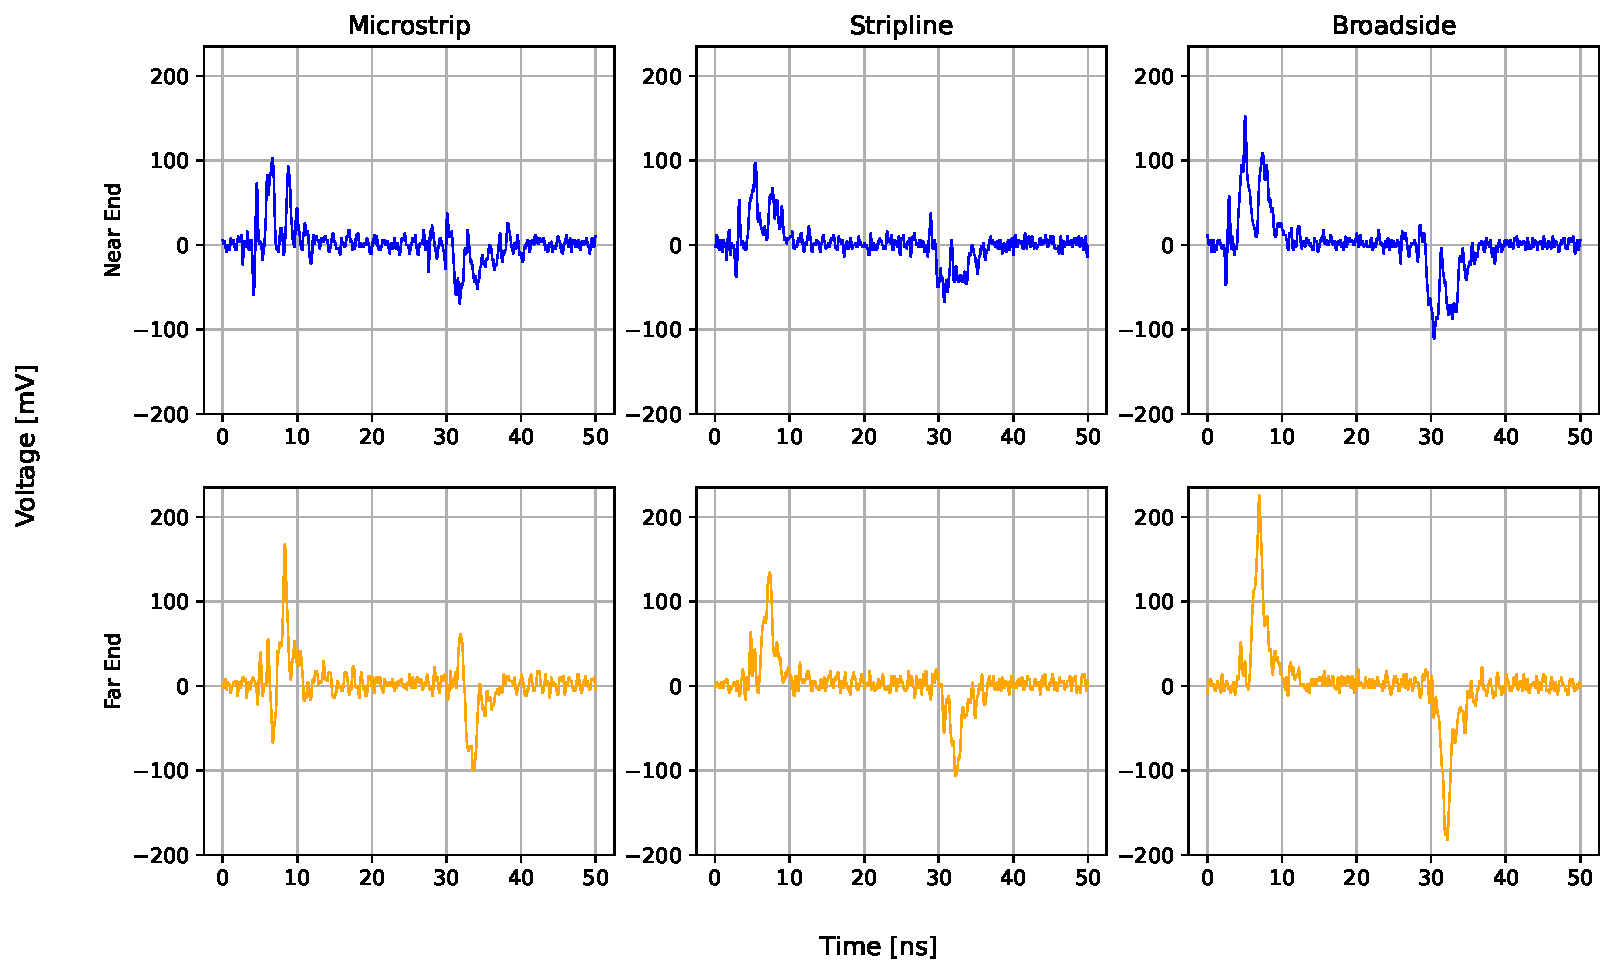
\includegraphics[width=1.0\textwidth]{measured_245v.pdf}
    \caption{Measured waveforms for the three transmission line configurations.}
    \label{fig:meas-waveforms2}
\end{figure}

\subsubsection{Crosstalk side-by-side microstrip}

\begin{table}[h]
    \centering
    \begin{tabular}{l l|r r}
        \toprule[1pt]
        \textbf{NEXT} & State & Steady State Level [mV] & Critical Level [mV] \\
        \midrule
        & Low State & 2.03 & 103 \\
        & High State & 3.31 & 3.23 \\
        \midrule[1pt]
        \textbf{FEXT} & State & Steady State Level [mV] & Critical Level [mV] \\
        \midrule
        & Low State & 3.75 & 168 \\
        & High State & 3.33 & 3.20 \\
        \bottomrule[1pt]
    \end{tabular}
    \caption{Crosstalk measurements for side-by-side microstrip.}
    \label{tab:meas-side-by-side-microstrip2}
\end{table}

\subsubsection{Crosstalk side-by-side stripline}

\begin{table}[h]
    \centering
    \begin{tabular}{l l|r r}
        \toprule[1pt]
        \textbf{NEXT} & State & Steady State Level [mV] & Critical Level [mV] \\
        \midrule
        & Low State & 1.77 & 96.8 \\
        & High State & 3.32 & 3.23 \\
        \midrule[1pt]
        \textbf{FEXT} & State & Steady State Level [mV] & Critical Level [mV] \\
        \midrule
        & Low State & 3.28 & 134 \\
        & High State & 3.32 & 3.19 \\
        \bottomrule[1pt]
    \end{tabular}
    \caption{Crosstalk measurements for side-by-side stripline.}
    \label{tab:meas-side-by-side-stripline2}
\end{table}

\subsubsection{Crosstalk broadside stripline}

\begin{table}[h]
    \centering
    \begin{tabular}{l l|r r}
        \toprule[1pt]
        \textbf{NEXT} & State & Steady State Level [mV] & Critical Level [mV] \\
        \midrule
        & Low State & 2.90 & 152 \\
        & High State & 3.32 & 3.19 \\
        \midrule[1pt]
        \textbf{FEXT} & State & Steady State Level [mV] & Critical Level [mV] \\
        \midrule
        & Low State & 3.91 & 225 \\
        & High State & 3.31 & 3.12 \\
        \bottomrule[1pt]
    \end{tabular}
    \caption{Crosstalk measurements for broadside stripline.}
    \label{tab:meas-broadside-stripline2}
\end{table}

\end{document}
